\begin{figure}[ht]
\begin{center}
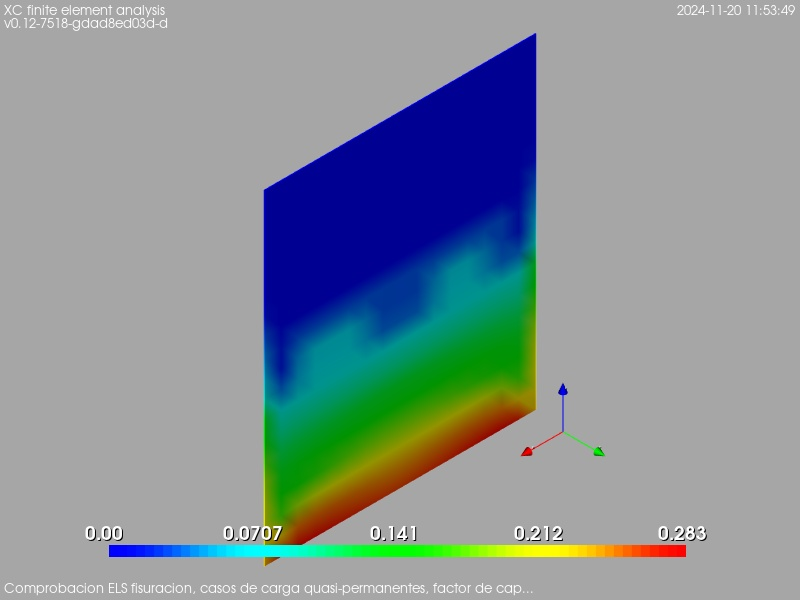
\includegraphics[width=\linewidth]{results/graphics/crackingSLS_qperm/wallCFSect1}
\caption{Comprobación ELS fisuración, casos de carga quasi-permanentes. Wall, factor de capacidad, dir. 1}
\label{SLS_quasiPermanentLoadsCrackControlwallCFSect1}
\end{center}
\end{figure}
\begin{figure}[ht]
\begin{center}
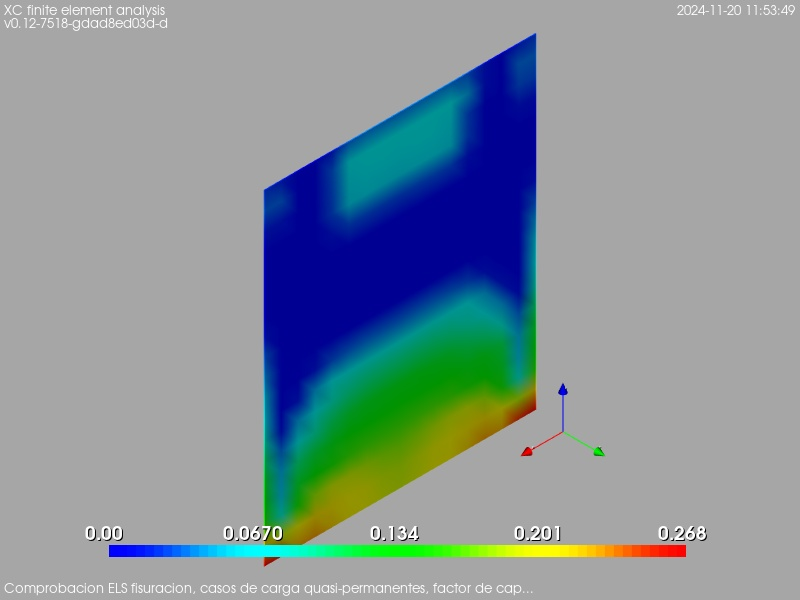
\includegraphics[width=\linewidth]{results/graphics/crackingSLS_qperm/wallCFSect2}
\caption{Comprobación ELS fisuración, casos de carga quasi-permanentes. Wall, factor de capacidad, dir. 2}
\label{SLS_quasiPermanentLoadsCrackControlwallCFSect2}
\end{center}
\end{figure}
\begin{figure}[ht]
\begin{center}
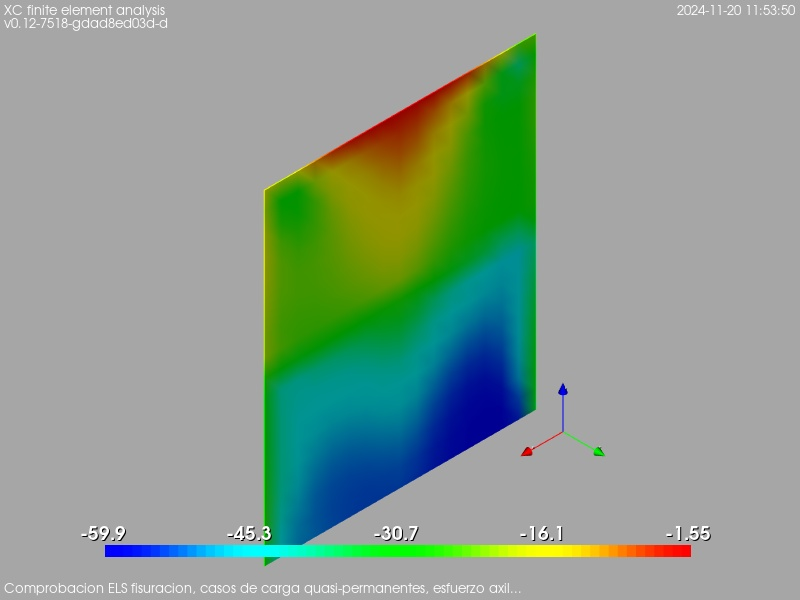
\includegraphics[width=\linewidth]{results/graphics/crackingSLS_qperm/wallNSect1}
\caption{Comprobación ELS fisuración, casos de carga quasi-permanentes. Wall, esfuerzo axil asociado al factor de capacidad, dir. 1}
\label{SLS_quasiPermanentLoadsCrackControlwallNSect1}
\end{center}
\end{figure}
\begin{figure}[ht]
\begin{center}
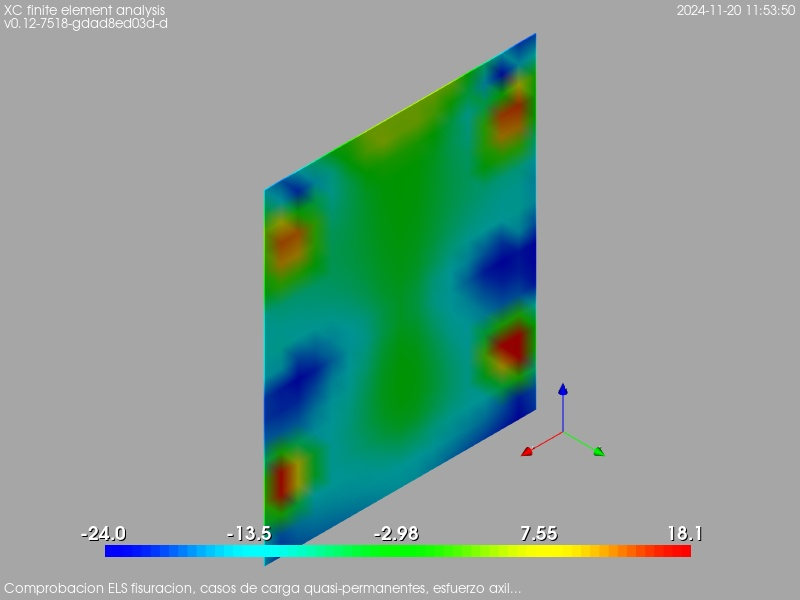
\includegraphics[width=\linewidth]{results/graphics/crackingSLS_qperm/wallNSect2}
\caption{Comprobación ELS fisuración, casos de carga quasi-permanentes. Wall, esfuerzo axil asociado al factor de capacidad, dir. 2}
\label{SLS_quasiPermanentLoadsCrackControlwallNSect2}
\end{center}
\end{figure}
\begin{figure}[ht]
\begin{center}
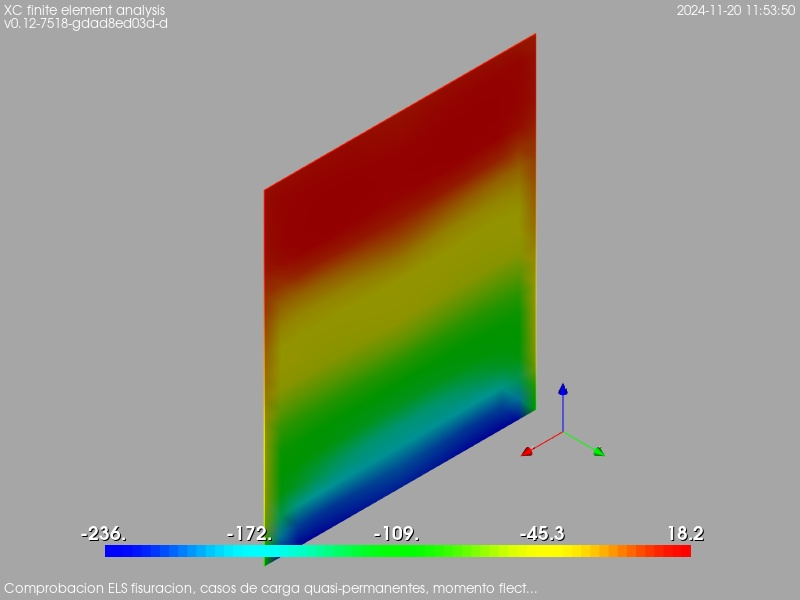
\includegraphics[width=\linewidth]{results/graphics/crackingSLS_qperm/wallMySect1}
\caption{Comprobación ELS fisuración, casos de carga quasi-permanentes. Wall, momento flector My asociado al factor de capacidad, dir. 1}
\label{SLS_quasiPermanentLoadsCrackControlwallMySect1}
\end{center}
\end{figure}
\begin{figure}[ht]
\begin{center}
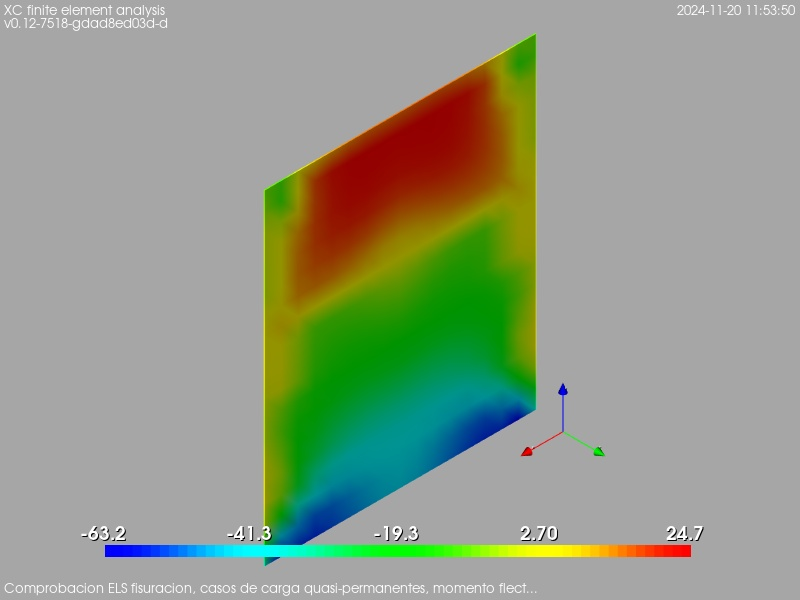
\includegraphics[width=\linewidth]{results/graphics/crackingSLS_qperm/wallMySect2}
\caption{Comprobación ELS fisuración, casos de carga quasi-permanentes. Wall, momento flector My asociado al factor de capacidad, dir. 2}
\label{SLS_quasiPermanentLoadsCrackControlwallMySect2}
\end{center}
\end{figure}
\begin{figure}[ht]
\begin{center}
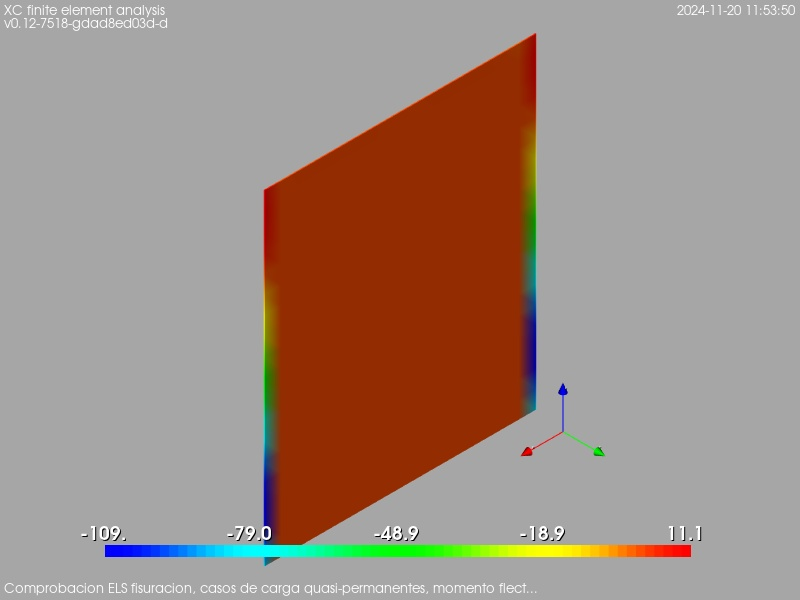
\includegraphics[width=\linewidth]{results/graphics/crackingSLS_qperm/wallMzSect1}
\caption{Comprobación ELS fisuración, casos de carga quasi-permanentes. Wall, momento flector Mz asociado al factor de capacidad, dir. 1}
\label{SLS_quasiPermanentLoadsCrackControlwallMzSect1}
\end{center}
\end{figure}
\begin{figure}[ht]
\begin{center}
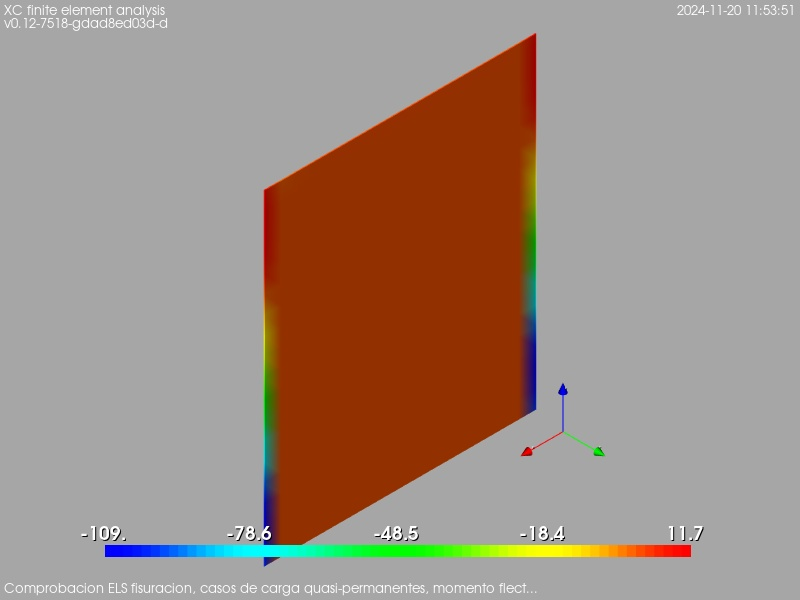
\includegraphics[width=\linewidth]{results/graphics/crackingSLS_qperm/wallMzSect2}
\caption{Comprobación ELS fisuración, casos de carga quasi-permanentes. Wall, momento flector Mz asociado al factor de capacidad, dir. 2}
\label{SLS_quasiPermanentLoadsCrackControlwallMzSect2}
\end{center}
\end{figure}
\begin{figure}[ht]
\begin{center}
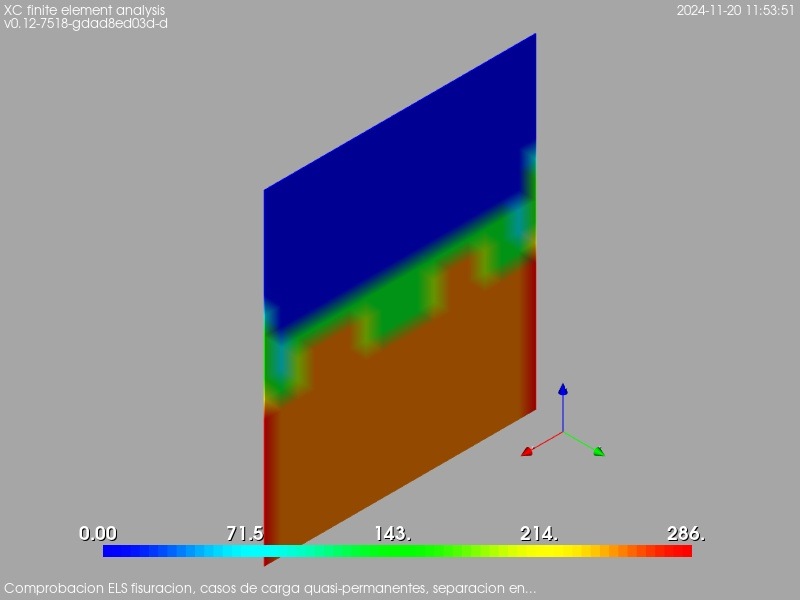
\includegraphics[width=\linewidth]{results/graphics/crackingSLS_qperm/walls_rmaxSect1}
\caption{Comprobación ELS fisuración, casos de carga quasi-permanentes. Wall, separación entre fisuras, dir. 1}
\label{SLS_quasiPermanentLoadsCrackControlwalls_rmaxSect1}
\end{center}
\end{figure}
\begin{figure}[ht]
\begin{center}
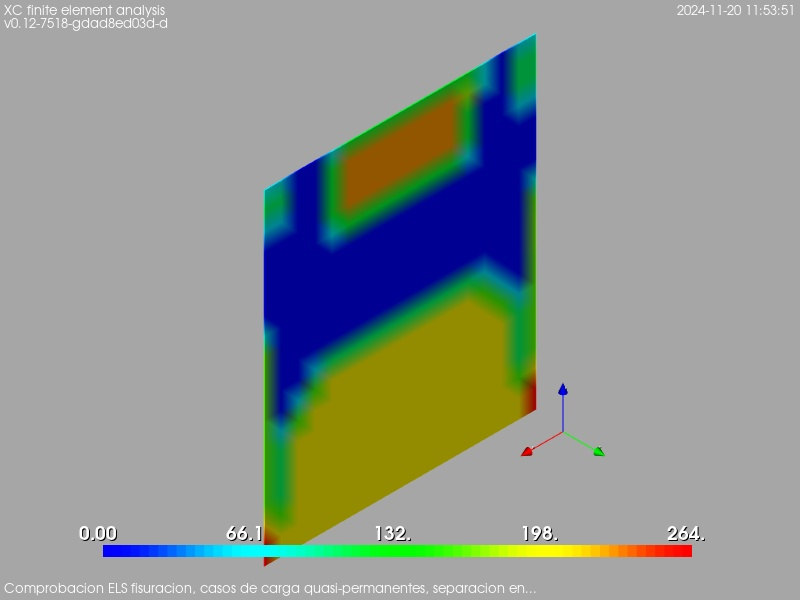
\includegraphics[width=\linewidth]{results/graphics/crackingSLS_qperm/walls_rmaxSect2}
\caption{Comprobación ELS fisuración, casos de carga quasi-permanentes. Wall, separación entre fisuras, dir. 2}
\label{SLS_quasiPermanentLoadsCrackControlwalls_rmaxSect2}
\end{center}
\end{figure}
\begin{figure}[ht]
\begin{center}
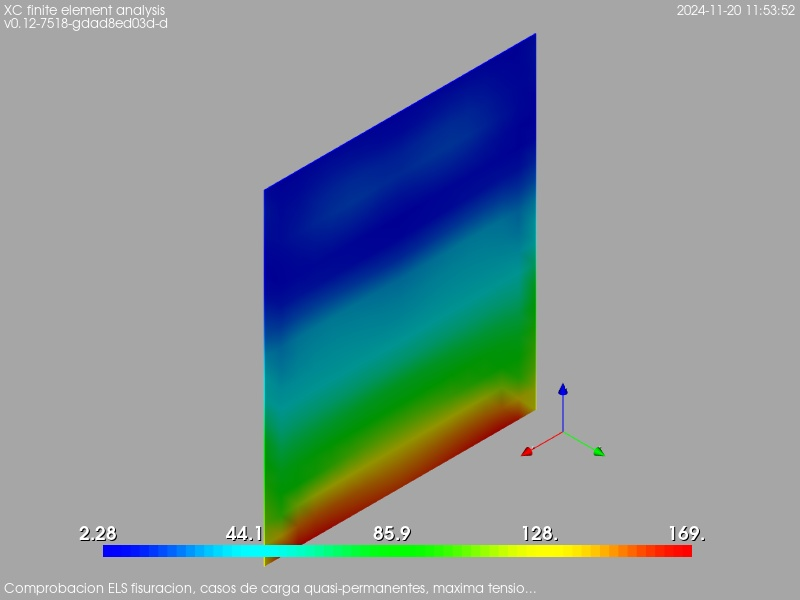
\includegraphics[width=\linewidth]{results/graphics/crackingSLS_qperm/wallsigma_sSect1}
\caption{Comprobación ELS fisuración, casos de carga quasi-permanentes. Wall, máxima tensión en la armadura, dir. 1}
\label{SLS_quasiPermanentLoadsCrackControlwallsigma_sSect1}
\end{center}
\end{figure}
\begin{figure}[ht]
\begin{center}
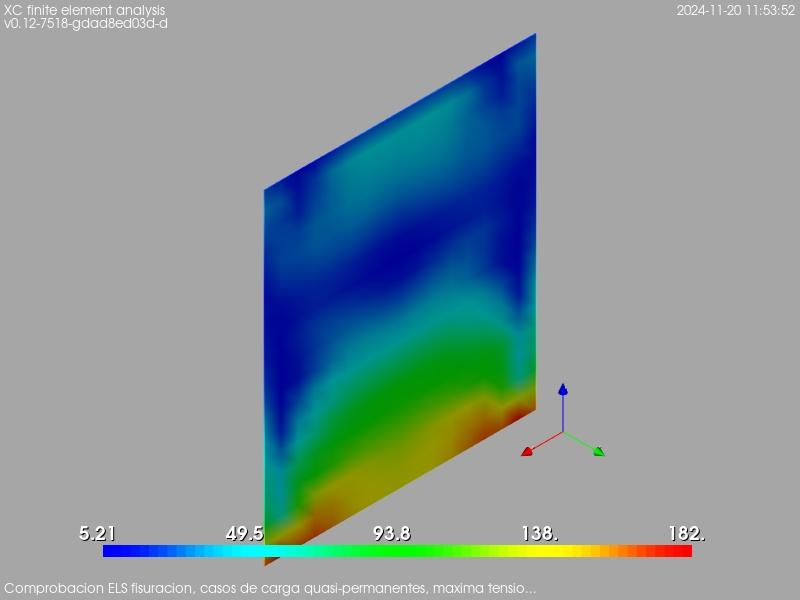
\includegraphics[width=\linewidth]{results/graphics/crackingSLS_qperm/wallsigma_sSect2}
\caption{Comprobación ELS fisuración, casos de carga quasi-permanentes. Wall, máxima tensión en la armadura, dir. 2}
\label{SLS_quasiPermanentLoadsCrackControlwallsigma_sSect2}
\end{center}
\end{figure}
\begin{figure}[ht]
\begin{center}
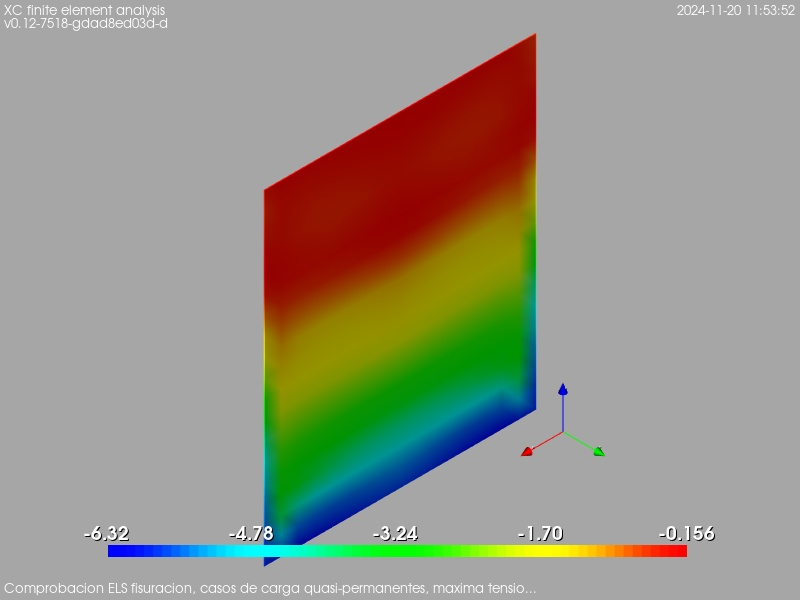
\includegraphics[width=\linewidth]{results/graphics/crackingSLS_qperm/wallsigma_cSect1}
\caption{Comprobación ELS fisuración, casos de carga quasi-permanentes. Wall, máxima tensión de compresión en el hormigón, dir. 1}
\label{SLS_quasiPermanentLoadsCrackControlwallsigma_cSect1}
\end{center}
\end{figure}
\begin{figure}[ht]
\begin{center}
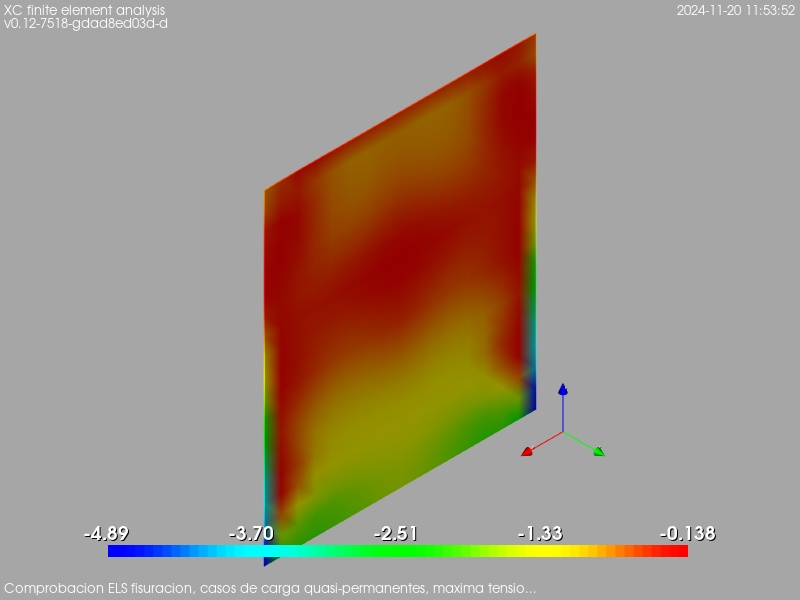
\includegraphics[width=\linewidth]{results/graphics/crackingSLS_qperm/wallsigma_cSect2}
\caption{Comprobación ELS fisuración, casos de carga quasi-permanentes. Wall, máxima tensión de compresión en el hormigón, dir. 2}
\label{SLS_quasiPermanentLoadsCrackControlwallsigma_cSect2}
\end{center}
\end{figure}
\begin{figure}[ht]
\begin{center}
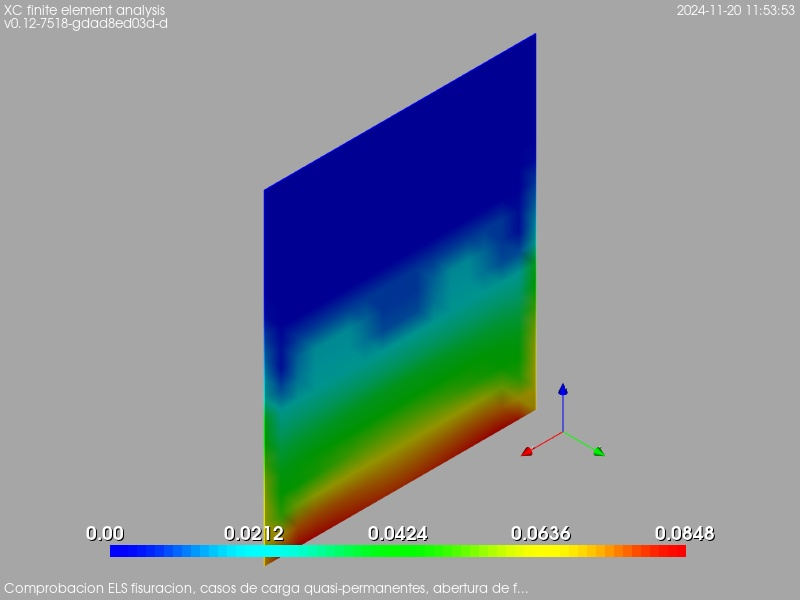
\includegraphics[width=\linewidth]{results/graphics/crackingSLS_qperm/wallwkSect1}
\caption{Comprobación ELS fisuración, casos de carga quasi-permanentes. Wall, abertura de fisura, dir. 1}
\label{SLS_quasiPermanentLoadsCrackControlwallwkSect1}
\end{center}
\end{figure}
\begin{figure}[ht]
\begin{center}
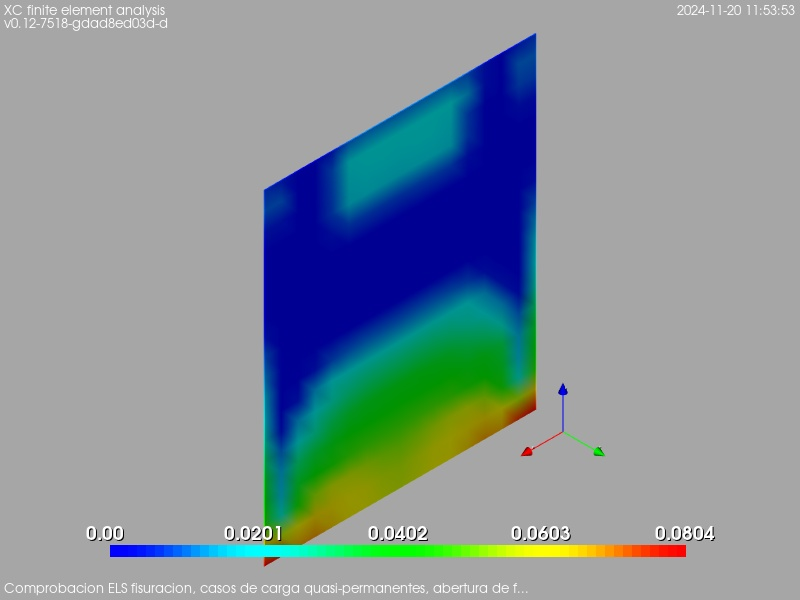
\includegraphics[width=\linewidth]{results/graphics/crackingSLS_qperm/wallwkSect2}
\caption{Comprobación ELS fisuración, casos de carga quasi-permanentes. Wall, abertura de fisura, dir. 2}
\label{SLS_quasiPermanentLoadsCrackControlwallwkSect2}
\end{center}
\end{figure}
\begin{figure}[ht]
\begin{center}
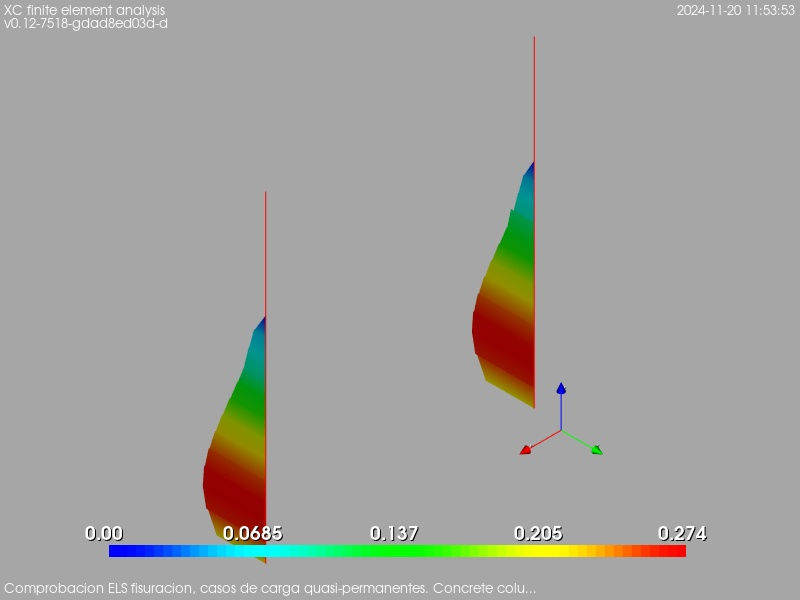
\includegraphics[width=\linewidth]{results/graphics/crackingSLS_qperm/columnZconcrCF}
\caption{Comprobación ELS fisuración, casos de carga quasi-permanentes. Concrete columns, factor de capacidad}
\label{SLS_quasiPermanentLoadsCrackControlcolumnZconcrCF}
\end{center}
\end{figure}
\begin{figure}[ht]
\begin{center}
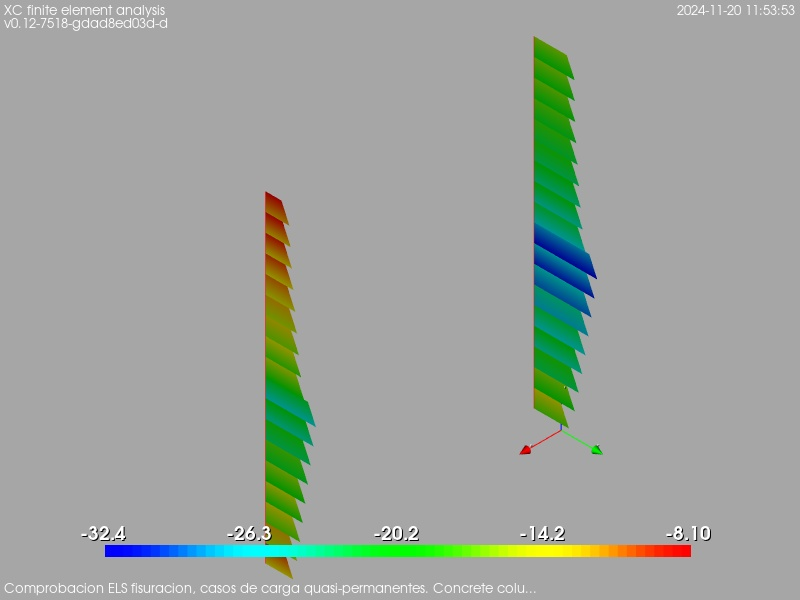
\includegraphics[width=\linewidth]{results/graphics/crackingSLS_qperm/columnZconcrN}
\caption{Comprobación ELS fisuración, casos de carga quasi-permanentes. Concrete columns, esfuerzo axil asociado al factor de capacidad}
\label{SLS_quasiPermanentLoadsCrackControlcolumnZconcrN}
\end{center}
\end{figure}
\begin{figure}[ht]
\begin{center}
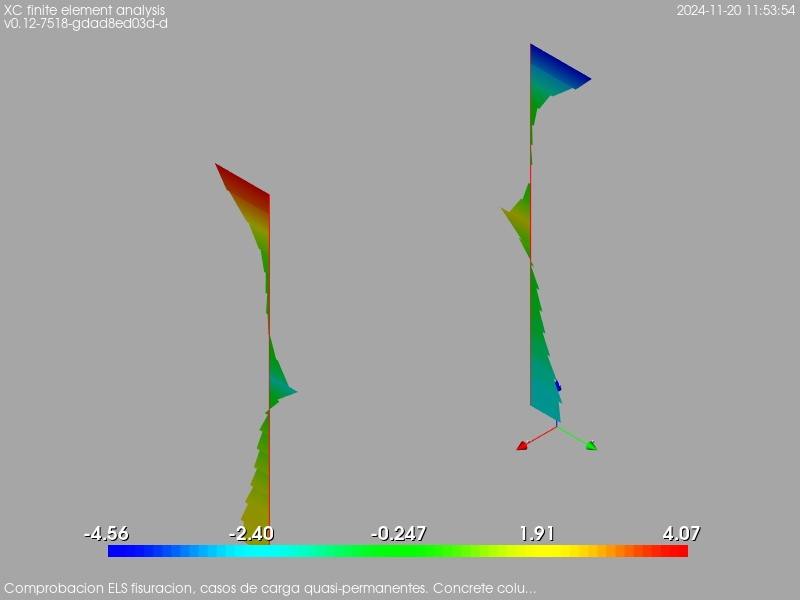
\includegraphics[width=\linewidth]{results/graphics/crackingSLS_qperm/columnZconcrMy}
\caption{Comprobación ELS fisuración, casos de carga quasi-permanentes. Concrete columns, momento flector My asociado al factor de capacidad}
\label{SLS_quasiPermanentLoadsCrackControlcolumnZconcrMy}
\end{center}
\end{figure}
\begin{figure}[ht]
\begin{center}
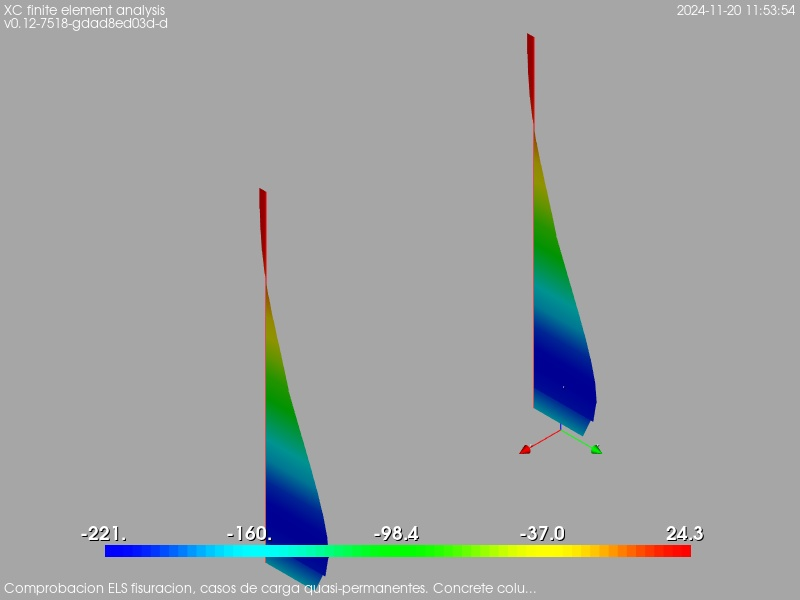
\includegraphics[width=\linewidth]{results/graphics/crackingSLS_qperm/columnZconcrMz}
\caption{Comprobación ELS fisuración, casos de carga quasi-permanentes. Concrete columns, momento flector Mz asociado al factor de capacidad}
\label{SLS_quasiPermanentLoadsCrackControlcolumnZconcrMz}
\end{center}
\end{figure}
\begin{figure}[ht]
\begin{center}
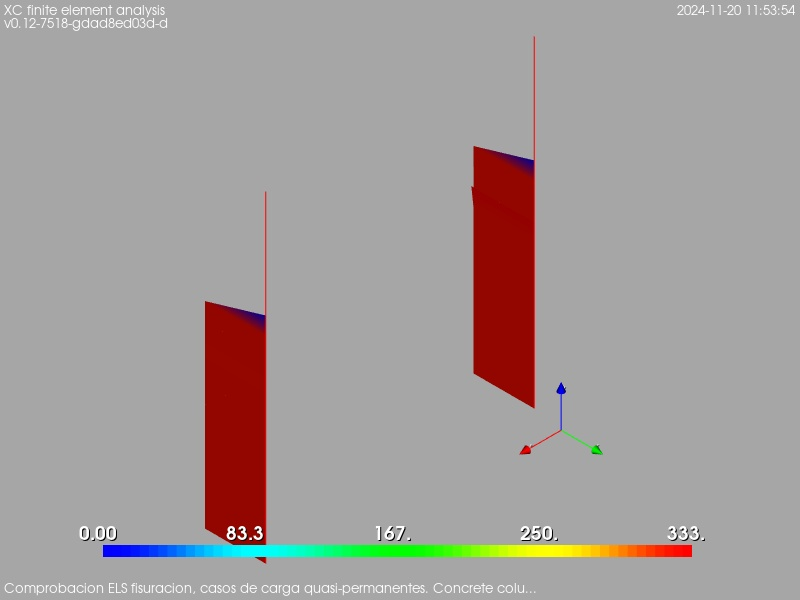
\includegraphics[width=\linewidth]{results/graphics/crackingSLS_qperm/columnZconcrs_rmax}
\caption{Comprobación ELS fisuración, casos de carga quasi-permanentes. Concrete columns, separación entre fisuras}
\label{SLS_quasiPermanentLoadsCrackControlcolumnZconcrs_rmax}
\end{center}
\end{figure}
\begin{figure}[ht]
\begin{center}
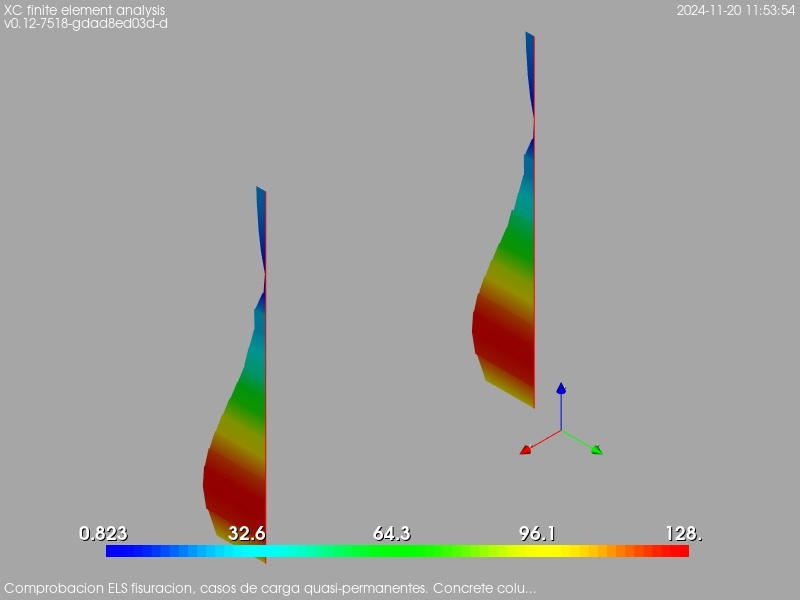
\includegraphics[width=\linewidth]{results/graphics/crackingSLS_qperm/columnZconcrsigma_s}
\caption{Comprobación ELS fisuración, casos de carga quasi-permanentes. Concrete columns, máxima tensión en la armadura}
\label{SLS_quasiPermanentLoadsCrackControlcolumnZconcrsigma_s}
\end{center}
\end{figure}
\begin{figure}[ht]
\begin{center}
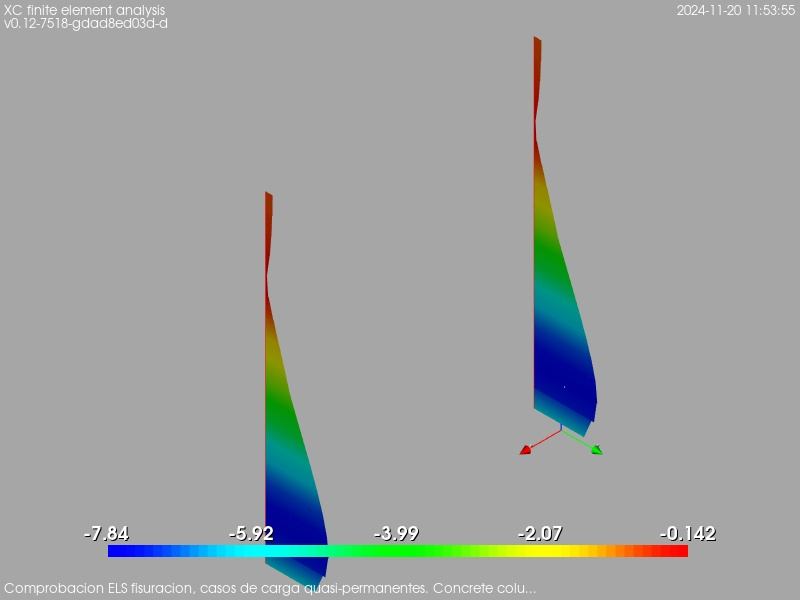
\includegraphics[width=\linewidth]{results/graphics/crackingSLS_qperm/columnZconcrsigma_c}
\caption{Comprobación ELS fisuración, casos de carga quasi-permanentes. Concrete columns, máxima tensión de compresión en el hormigón}
\label{SLS_quasiPermanentLoadsCrackControlcolumnZconcrsigma_c}
\end{center}
\end{figure}
\begin{figure}[ht]
\begin{center}
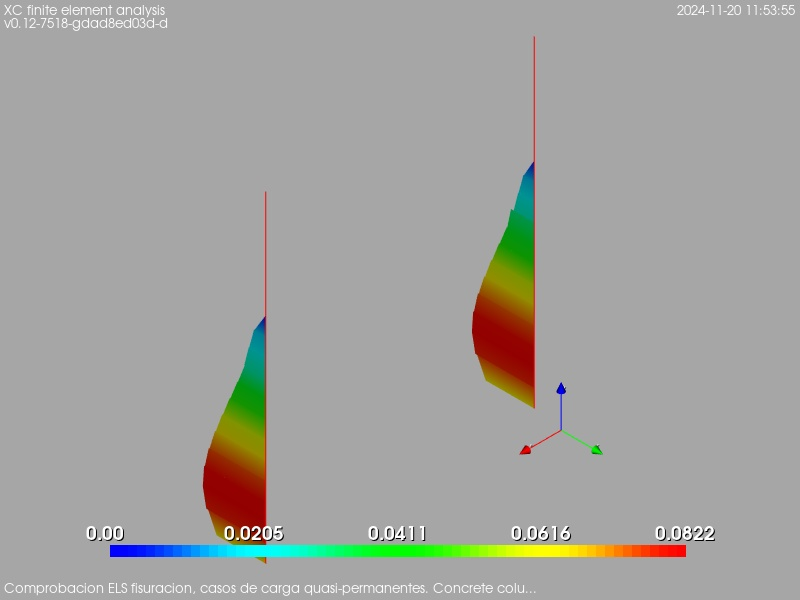
\includegraphics[width=\linewidth]{results/graphics/crackingSLS_qperm/columnZconcrwk}
\caption{Comprobación ELS fisuración, casos de carga quasi-permanentes. Concrete columns, abertura de fisura}
\label{SLS_quasiPermanentLoadsCrackControlcolumnZconcrwk}
\end{center}
\end{figure}
